\chapter{The Compost Bomb and the Terrestrial Carbon Cycle}
\label{chapter:global_bomb}
\graphicspath{{global_bomb/figs/}}

\todo[inline]{This is basically just going to be equations for now}


In \cref{chapter:continuous_compost_bomb} we saw how introducing a vertical dimension can affect the compost bomb.
We can also introduce horizontal dimensions into the problem. We therefore need to decide at what horizontal scale we
should work. We will work at the global-averaged scale motivated by work \parencite{Cox2006} which suggests a instability in the global
carbon cycle in certain parameter regimes. How does biogeochemical feedback affect this instability?

Following \cite{Luke2011}, we have the compost bomb equations
\begin{subequations}
  \label{eq:compost_bomb_equations}
  \begin{align}
    \mu \dv{T_s}{t} &= - \kappa \left(T_s - T_a\right) + Ar_0C_se^{\alpha T_s} \label{eq:compost_bomb_soil_temperature} \\
    \dv{C_s}{t} &= \Pi - r_0C_se^{\alpha T_s} \label{eq:compost_bomb_soil_carbon}
  \end{align}
\end{subequations}

Noting the obvious timescale seperation in \cref{eq:compost_bomb_equations} we can put \cref{eq:compost_bomb_soil_temperature} into
equilibrium to get
\begin{equation*}
  0 = - \kappa \left(T_s - T_a\right) + Ar_0C_se^{\alpha T_s}
\end{equation*}
which can be solved for the soil temperature to  give
\begin{equation}
  \label{eq:soil_temperature_equilibrium}
  T_s = T_a - \frac{1}{\alpha} W\left(-\frac{Ar_0C_s \alpha e^{\alpha T_a}}{\kappa} \right),
\end{equation}
where $W(x)$ is the Lambert $W$ function. The Lambert $W$ function, plotted in \cref{fig:lambert_W}, is defined as the solution to the equation
\begin{equation}
  \label{eq:lambert_W}
  W(x)e^{W(x)} = x.
\end{equation}

\begin{figure}
  \centering
  \begin{tikzpicture}
    \begin{axis}[
      xmin=-1,
      xmax=4,
      enlarge y limits=false,
      axis lines=left,
      xlabel=$x$,
      ylabel=$W(x)$,
      samples=50]
      \addplot[domain=-5:-1] (x * exp(x), x);
      \addplot[domain=-1:2] (x * exp(x), x);
    \end{axis}
  \end{tikzpicture}
  \caption{The Lambert $W$ function}
  \label{fig:lambert_W}
\end{figure}

Defining
\begin{equation}
  \label{eq:critical_npp}
  \Pi_c = \frac{\kappa}{\alpha A}
\end{equation}
we can rewrite \cref{eq:soil_temperature_equilibrium} as
\begin{equation}
  \label{eq:soil_temperature_equilibrium_nppc}
  T_s = T_a - \frac{1}{\alpha} W\left(-\frac{r_0C_s e^{\alpha T_a}}{\Pi_c} \right).
\end{equation}
We should therefore insert \cref{eq:soil_temperature_equilibrium_nppc} in \cref{eq:compost_bomb_soil_carbon}
to give
\begin{equation}
  \label{eq:soil_carbon_evolution}
  \dv{C_s}{t} = \Pi + \Pi_c W\left(-\frac{r_0C_s e^{\alpha T_a}}{\Pi_c} \right).
\end{equation}
This implies the equilibrium value of $C_s$ is
\begin{equation}
  \label{eq:equilibirum_soil_carbon}
  C_s^{\mathrm{eq}} = \frac{\Pi}{r_0} e^{-\alpha T_a} e^{-\Pi/\Pi_c}.
\end{equation}
Note that we recover the no biogeochemcial heating case by sending $\Pi_c \rightarrow \infty$.


Recognising that
\begin{equation}
  \label{eq:atmospheric_temperatures}
  T_a = \frac{S}{\log 2} \log \frac{C_a}{C_{a0}} 
\end{equation}
leads, upon substituting \cref{eq:atmospheric_temperatures} into \cref{eq:soil_carbon_evolution},
\begin{equation}
  \label{eq:global_soil_carbon}
  \dv{C_s}{t} = \Pi + \Pi_c W\left(-\frac{r_0C_s}{\Pi_c} \left(\frac{C_a}{C_{a0}}\right)^\mu \right),
\end{equation}
where
\begin{equation}
  \label{eq:mu}
  \mu = \frac{\alpha S}{\log 2}.
\end{equation}


We chose the temperature anomaly so that $T_a = 0$ corresponds to an equilibrium. We can then set
$r_0 = \frac{\Pi_0}{C_s^{\mathrm{eq}}}e^{-\Pi_0/\Pi_c}$, where $\Pi_0 = \Pi\left(C_{a0}\right)$.

To
numerically compute the equilibria of \cref{eq:global_soil_carbon} we need to define the dependence of $\Pi$ on
$C_a$  and the dependence of $C_a$ on $C_s$. We set NPP to
\begin{equation}
  \label{eq:npp_fertilization}
  \Pi(C_a) = \frac{\Pi_{\infty} C_a}{C_a + C_{a_{1/2}}}.
\end{equation}
This is an increasing function of $C_a$, which saturates to $\Pi_{\infty}$ for $C_a \gg C_{a_{1/2}}$.
We will assume  that a fixed fraction $\chi_0$ of atmospheric emissions reaches the ocean, meaning
\begin{equation}
  \label{eq:simple_ocean}
  C_a = C_{a0} -\frac{1}{1+\chi_0} (C_s - C_{s}^{\mathrm{eq}}).
  %C_s = C_{s}^{\mathrm{eq}} - (1 + \chi_0)(C_a - C_{a0}.
\end{equation}
It is now straightforward to compute the bifurcation diagram, which we do in \todo{bifurcation diagram!} 
\missingfigure{Bifurcation Diagram of \cref{eq:global_soil_carbon}}

We can make analytic progress too. To find the bifurcation we therefore just have to calculate where
\begin{equation*}
  \dv{\dot{C_s}}{C_s} = 0,
\end{equation*}
we will make use of
\begin{equation}
  \label{eq:derivative_of_lambert_W}
  W'(x) = \frac{W(x)}{x\left(1 + W\left(x\right)\right)}.
\end{equation}




Taking a derivative of the right hand side of \cref{eq:global_soil_carbon} and setting it to zero in equilibrium gives
\begin{equation}
  \label{eq:soil_carbon_lambda}
  \dv{\Pi}{C_a}\dv{C_a}{C_s} + \frac{\Pi_c}{C_s^{\mathrm{eq}}} \frac{W\left(-\frac{r_0C_s^{\mathrm{eq}}}{\Pi_c}\right)}{1+W\left(-\frac{r_0C_s^{\mathrm{eq}}}{\Pi_c}\right)} \left(
    1 + \mu \frac{C_s^{\mathrm{eq}}}{C_{a0}} \dv{C_a}{C_s}\right) = 0
\end{equation}
so
\begin{equation}
  \label{eq:critical_mu}
  \mu = -\frac{C_{a0}}{C_{s}^{\mathrm{eq}}}\dv{C_s}{C_a}\left(\dv{\Pi}{C_a}\dv{C_a}{C_s} \frac{C_s^{\mathrm{eq}}}{\Pi_c}\frac{1+W\left(-\frac{r_0C_s^{\mathrm{eq}}}{\Pi_c}\right)}{W\left(-\frac{r_0C_s^{\mathrm{eq}}}{\Pi_c}\right)} + 1 \right)
\end{equation}
which simplifies to
\begin{equation}
  \label{eq:critical_mu_simple_ocean}
  \mu = \left(1+\chi_0\right) \frac{C_{a0}}{C_{s}^{\mathrm{eq}}} -
  \frac{C_{a0}}{\Pi_c}\frac{1+W\left(-\frac{r_0C_s^{\mathrm{eq}}}{\Pi_c}\right)}{W\left(-\frac{r_0C_s^{\mathrm{eq}}}{\Pi_c}\right)}\dv{\Pi}{C_a}.
\end{equation}
This can be further reduced to
\begin{equation*}
  \mu = \left(1+\chi_0\right) \frac{C_{a0}}{C_{s}^{\mathrm{eq}}} -
  \frac{C_{a0}}{\Pi_c}
  \frac{1+W\left(-\frac{\Pi_0}{\Pi_c}\exp\left(-\frac{\Pi_0}{\Pi_c}\right)\right)}
  {W\left(-\frac{\Pi_0}{\Pi_c}\exp\left(-\frac{\Pi_0}{\Pi_c}\right)\right)}\dv{\Pi}{C_a} 
\end{equation*}
and even more to give
\begin{equation*}
  \mu = \left(1+\chi_0\right) \frac{C_{a0}}{C_{s}^{\mathrm{eq}}} -
  \frac{C_{a0}}{\Pi_c}
  \frac{1-\frac{\Pi_0}{\Pi_c}}{-\frac{\Pi_0}{\Pi_c}}\dv{\Pi}{C_a}.
\end{equation*}
Cleaning this up gives the final form.
\begin{equation}
  \label{eq:critical_mu_simple_ocean_in_terms_of_npp}
  \mu^* = \left(1+\chi_0\right) \frac{C_{a0}}{C_{s}^{\mathrm{eq}}} +
  \frac{C_{a0}}{\Pi_0} \dv{\Pi}{C_a} - \frac{C_{a0}}{\Pi_c}\dv{\Pi}{C_a}.
\end{equation}
We remark that taking the limit where $\Pi_c \rightarrow \infty$ gives
\begin{equation}
  \label{eq:mu_infinity}
  \mu^*_{\infty} =\left(1+\chi_0\right) \frac{C_{a0}}{C_{s}^{\mathrm{eq}}} +
  \frac{C_{a0}}{\Pi_0} \dv{\Pi}{C_a}.
\end{equation}
This corresponds to the limit where biogeochemcial heating does not occur.

% We note this implies a minimum allowed \ce{CO2} fertilization effect for a given $\mu$ (as we need $\mu < \mu_\infty^*$)
% \begin{equation}
%   \label{eq:minimum_allowed_co2_fertilization}
%   \dv{\Pi}{C_a} > \frac{\Pi_0\mu}{C_{a0}} - \frac{1+\chi_0}{C_s^{\mathrm{eq}}}\Pi_0
% \end{equation}


We can plot \cref{eq:critical_mu} to devide the parameter plane into a stable and unstable region.

\begin{figure}
  \centering
  \begin{tikzpicture}[
    /pgf/declare function={
      chi0 = 0.25;
      npp = 55.0;
      Ca0 = 589.0;
      Cseq = 1500.0;
    }
    ]
    \begin{axis}[
      legend pos=outer north east,
      % enlargelimits=false
      xlabel={$\Pi_c$},
      ylabel={$\mu$},
      xmin=20,
      xmax=500,
      ymin=0.0
      ]
      \addplot[
      domain=20:500,
      samples=100,
      color=red]
      {(1+chi0)*Ca0/Cseq + 0.07 * ((Ca0/npp)  - (Ca0/x))};
      \addplot[
      domain=20:500,
      samples=100,
      color=red,
      dashed]
      {(1+chi0)*Ca0/Cseq + 0.07 * ((Ca0/npp))};
      \addlegendentry{$\dv*{\Pi}{C_a} = 0.07$}
    \end{axis}
  \end{tikzpicture}
  \caption{The parameter plane}
  \label{fig:critical_mu_vs_pic}
\end{figure}


\section{What is $S$?}
\todo[inline]{Can also look at respiration directly}
Ignoring the effects of biogeochemical heating, we can write spatially resolved soil carbon equations:
\begin{equation}
  \label{eq:spatially_resolved_soil_carbon}
  \pdv{ C_s (\bm{r},t)}{t} = \Pi(\bm{r},t) - r_0(\bm{r},t)C_s(\bm{r},t)e^{\alpha T(\bm{r},t)}
\end{equation}
Averaging gives
\begin{equation}
  \label{eq:spatially_averaged_soil_carbon}
  \dv{\left\langle C_s\right\rangle}{t} = \left\langle \Pi \right \rangle - \left\langle r_0 C_s e^{\alpha T} \right \rangle
\end{equation}
Expanding:
\begin{align*}
  \dv{\left\langle C_s\right\rangle}{t} &\approx \left\langle \Pi \right \rangle - \left\langle r_0 C_s + r_0 C_s \alpha T \right \rangle \\
                                        &\approx \left\langle \Pi \right \rangle - \left\langle r_0 C_s\right \rangle - \alpha \left \langle r_0C_s T\right\rangle \\
                                        &=\approx - \alpha \left \langle \Pi T\right\rangle,
\end{align*}
where we have used $\Pi = r_0C_s$ in equilibrium. Introducting an effective temperature $T_{\mathrm{eff}}$ we get
\begin{equation*}
  - \alpha \left \langle \Pi T \right\rangle = - \alpha \left \langle \Pi \right\rangle T_{\mathrm{eff}}
\end{equation*}
so that
\begin{equation}
  \label{eq:definition_of_effective_temperature}
  T_{\mathrm{eff}} = \frac{\left \langle \Pi T \right\rangle}{\left \langle \Pi \right\rangle}.
\end{equation}
After a double of \ce{CO2} we have $T_{\mathrm{eff}} = S$ and $\langle T \rangle = \mathrm{ECS}$ so that
\begin{equation}
  \label{eq:S_vs_ECS}
  \frac{S}{\mathrm{ECS}} = \frac{\left \langle \Pi T \right\rangle}{\left \langle \Pi \right\rangle \left \langle T \right \rangle}.
\end{equation}
In words, $S$ is given by an NPP weighted average of global temperatures.
Based on HADGEM2-ES CMIP5 abrupt $4\times\ce{CO2}$ runs, we get $S/\mathrm{ECS} \approx 1.6$.
\section{What is $\Pi_c$?}
\todo[inline]{Do with Physically based --- with Penman Monteith - this is giving me a constraint on the ratio?}
To get a reasonable estimate of $\Pi_c$, we need $\alpha$, $A$ and $\kappa$. With a value of $Q_{10} \approx 2$, we find $\alpha \approx 0.03$.
We take $A$ from biochemistry to be \SI{3.9E7}{\joule\per\kilo\gram\carbon}. To estimate $\kappa$, we neglect biogeochemical heating
in \ref{eq:compost_bomb_soil_temperature} to get
\begin{equation}
  \label{eq:soil_temp_no_biogeo}
  \mu \dot{T_s} = -\kappa \left( T_s -T_a \right)
\end{equation}
and then move to the frequency domain by fourier transforming to get power spectrum of $T_s$ in terms of $T_a$
\begin{equation}
  \label{eq:power_spectrum_of_Ts}
  \left| \tilde{T}_s\left(\omega\right)\right|^2 = \frac{\kappa^2 \left| \tilde{T}_a\left(\omega\right)\right|^2}{\omega^2 \mu^2 + \kappa^2}.
    \end{equation}
Estimates of $\kappa$ and $\mu$ can therefore be extracted from timeseries of global $T_a$ and $T_s$ giving $\kappa$ to be \SI{0.27}{\watt\per\meter}\todo{check units}
and so $\Pi_c \approx$ \SI{300}{\kilo\gram\carbon\per\year}\todo{check}

\section{Variability and Autocorrelation}
\begin{figure}
  \centering
  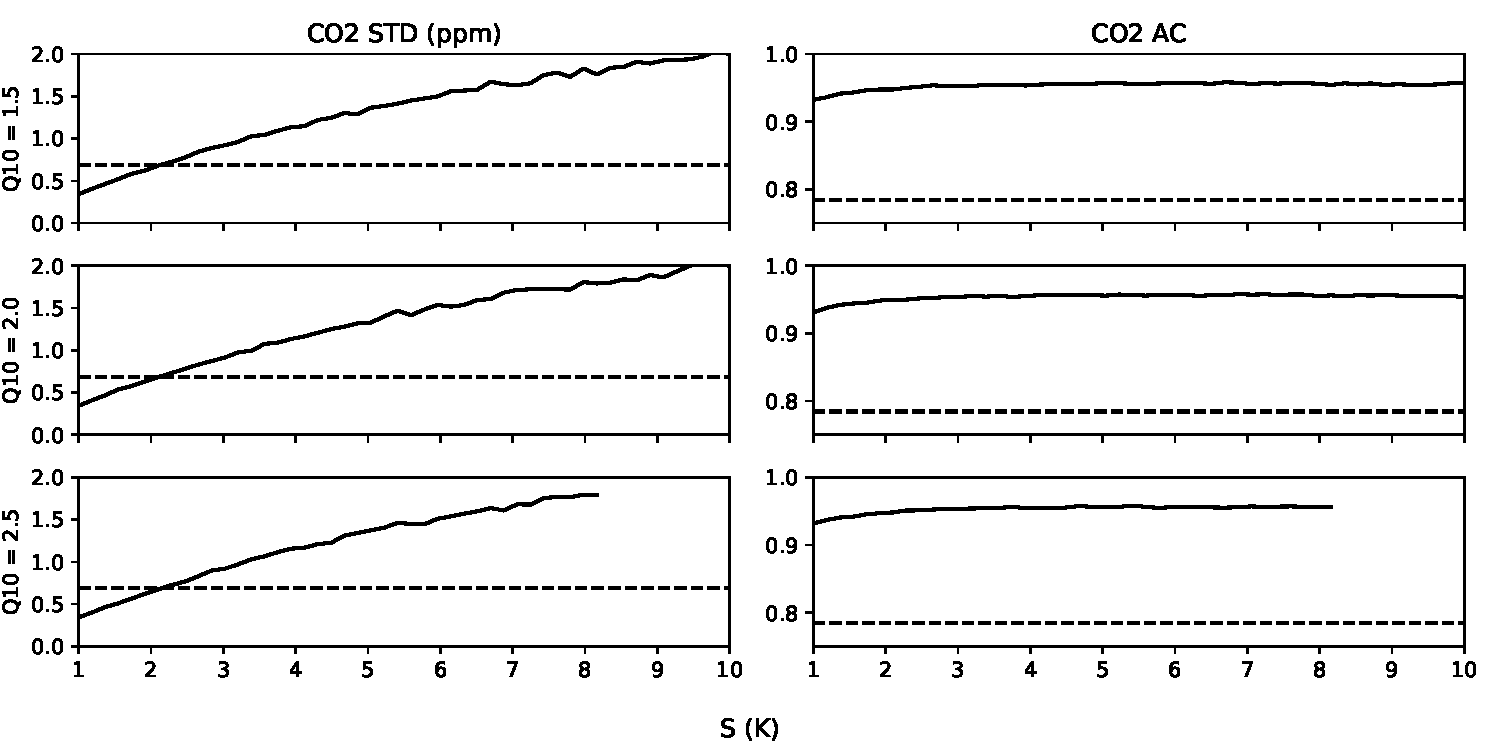
\includegraphics[width=\textwidth]{co2_std_ac}
  \caption[Atmospheric Carbon Variability]{Standard Deviation and Autocorrelation of atmospheric carbon}
  \label{fig:co2_std_ac}
  \end{figure}\todo{do this instead with more complex model}
  \begin{figure}
  \centering
  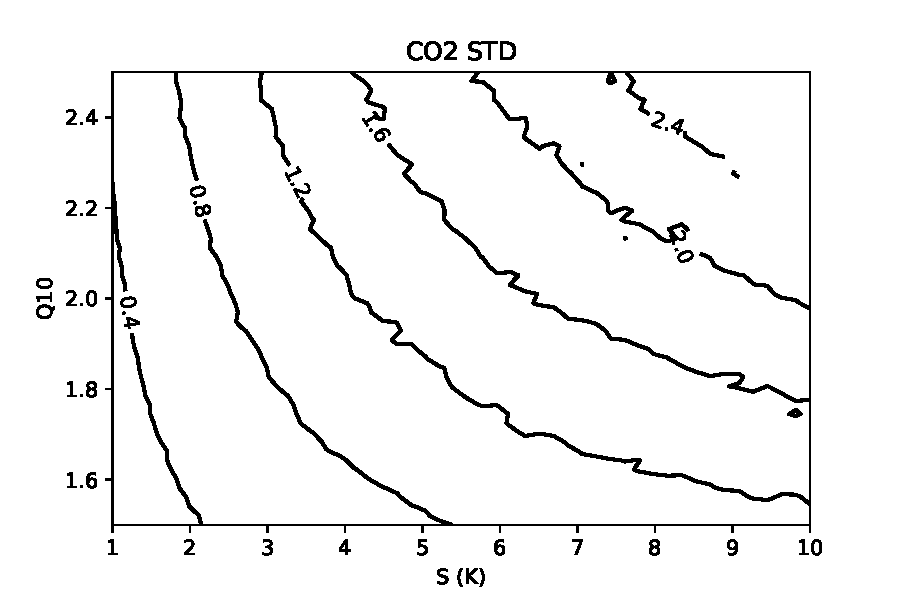
\includegraphics{co2stdcontour}
  \caption{CO2 standard deviation}
  \label{fig:co2_std_Q10_S}
\end{figure}
\begin{figure}
  \centering
  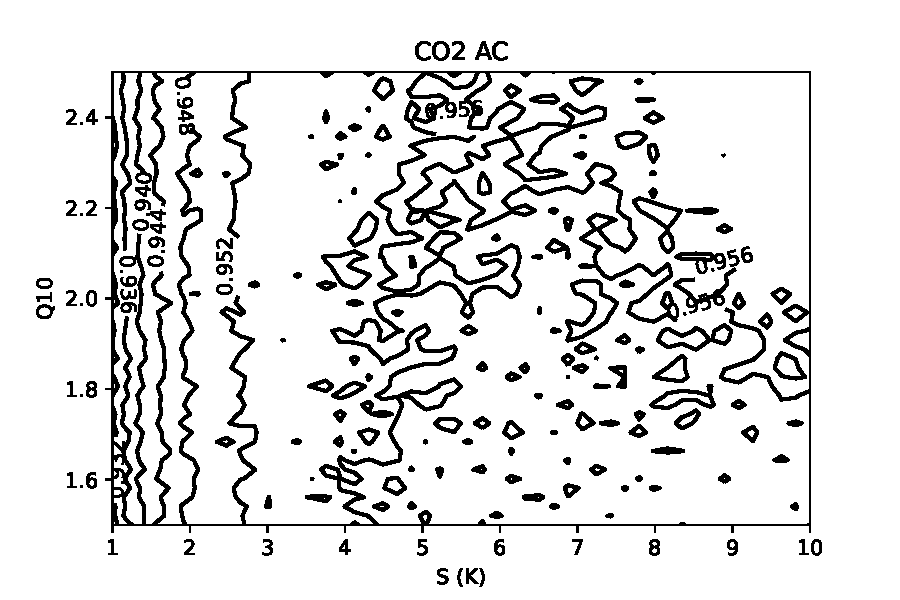
\includegraphics{co2accontour}
  \caption{CO2 AC}
  \label{fig:co2_ac_Q10_S}
\end{figure}
\section{A more Realistic Ocean Model}
\todo[inline]{Split into two chapters here?}
\subsection{A dynamic Ocean Box}
Assume only one ocean box which responds linearly to elevated atmospheric \ce{CO2}. Set the
total carbon in the atmosphere-land-ocean system to $\mathcal{C}$.

Work with the system:
\begin{subequations}
  \label{eq:one_box_ocean}
  \begin{align}
    \dv{C_s}{t} &= \Pi(C_a) - r_0 C_s \left(\frac{C_a}{C_{a0}}\right)^{\mu} \\
    \dv{C_o}{t} &= k(C_a - C_{a0}) - \frac{C_o}{\tau} \\
    C_a &= \mathcal{C} - C_s - C_o
\end{align}
\end{subequations}
This leads to the Jacobian:
\begin{equation}
  \label{eq:jacobian_of_one_box}
    \bm{J} = 
    \begin{pmatrix}
    r_0 \left( \mu \frac{C_{s0}}{C_{a0}} - 1\right) - \Pi'(C_{a0}) & 
    \mu \frac{C_{s0}}{C_{a0}} - \Pi'(C_{a0}) \\
    -k & -k - \frac{1}{\tau}
    \end{pmatrix}
\end{equation}
To find the eigenvalues, we need to find the roots of the characteristic polynomial:
$\det(\bm{J} - \gamma \bm{I})$ = 0, where $\gamma$ is an eigenvalue. This equation is quadratic with 
two roots. Solving it leads to:
\begin{equation}
  \label{eq:eigenvalues_of_one_box_jac}
  \gamma_{\pm} = \frac{B \pm \sqrt{\Delta}}{2\tau C_{a0}}
\end{equation}
where
\begin{equation}
  \label{eq:B_in_one_box}
  B = -k \tau  C_{a0}-\Pi'(C_{a0}) \tau  C_{a0}-r_0 \tau  C_{a0}-C_{a0}+\mu  \Pi_0 \tau
\end{equation}
and
\begin{equation}
  \label{eq:discriminant_from_one_box}
  \Delta = \left(k \tau  C_{a0} +\Pi'\tau  C_{a0}+r_0 \tau  C_{a0}+C_{a0}-\mu  \Pi_0 \tau \right)^2-4 \left(k r_0 \tau ^2 C_{a0}^2+\Pi' \tau  C_{a0}^2-\mu  \Pi_0 \tau  C_{a0} +r_0 \tau  C_{a0}^2\right)
\end{equation}
is the determinant. I have used $\Pi_0 = r_0 C_{s0}$.

The behaviour of this system will depend on the sign of $\Delta$.

\subsubsection{Real Eigenvalues}
If $\tau < 1/r_0$ then $\Delta > 0$ for all values of $\mu$. $1/r_0 \approx 30$ years so this represents the fast ocean response.
To find the instability, we look for when $\gamma_+ > 0$. Under the assumption of a fast ocean response,
\begin{equation}
  \label{eq:instability_condition_one_box_fast}
  \mu^* = \frac{C_{a0}}{C_{s0}} + \frac{C_{a0}}{\Pi_0} \dv{\Pi}{C_a} + \frac{C_{a0}}{C_{s0}} k\tau.
\end{equation}
This is essentially the condition in \cref{eq:mu_infinity} if we make the identification $\chi_0 = k \tau$.
\subsubsection{Complex Eigenvalues}
If $\Delta < 0$, which is to say if the ocean response is considered on a long timescale, the stabilty of the system is given by the sign of $B$.
This leads to the condition
\begin{equation}
  \label{eq:instability_condition_one_box_slow}
  \mu^* =\frac{C_{a0}}{C_{s0}} + \frac{C_{a0}}{\Pi_0} \dv{\Pi}{C_a} + \frac{C_{a0}}{C_{s0}} k\tau\left(
     1 + \frac{1}{k\tau}
  \right) \frac{1}{r_0\tau}
\end{equation}
This corresponds to the eigenvalues crossing the imaginary axis and is thus a Hopf bifurcation.
\subsection{Two Dynamic Ocean Boxes}
Suppose I modify \cref{eq:one_box_ocean} to include an extra ocean box. I imagine a fast box and a slow box. In principle, I could repeat the
analysis above, by finding the eigenvalues of a $3 \times 3$ matrix. This is possible in principle but involves solving a cubic polynomial which
is challenging analytically.

Instead, I will use the timescale seperation between the two ocean boxes to make some remarks about the qualitative behaviour of the system.
As the slow box is much slower than the fast box, over short timescales it can be ignored. So if $\mu$ were to be slowly increased through
the condition given in \cref{eq:instability_condition_one_box_fast} there would still be an instability.

However, on longer timescales, the system will still behave like a one box model but now the box will be the slow ocean component. As this is the slow box,
it will have $\Delta < 0$ and so there will be oscillatory behaviour. Hence I expect the bifurcation to occur at a similar place as in the one box fast ocean model,
but to have the character of a Hopf bifurcation.

To be more formal, consider the system
\begin{subequations}
  \begin{align}
    \label{eq:two_box_ocean}
    \dv{C_s}{t} &= \Pi(C_a) - r_0 C_s \left(\frac{C_a}{C_{a0}}\right)^{\mu} \\
    \dv{C_1}{t} &= fk(C_a - C_{a0}) - \frac{C_1}{\tau} \\
    \dv{C_2}{t} &= (1-f)k(C_a-C_{a0}) - \epsilon\frac{C_2}{\tau} \\
    C_a &= \mathcal{C} - C_s - C_1 - C_2
  \end{align}
\end{subequations}
where $f$ is the fraction of carbon taken up by the fast response and $\epsilon$ is the ratio of the timescale of the fast box to the slow box, so $\epsilon \ll 1$. If
$C_2$ can be taken as approximately constant, then there is an instability when $\mu^*_{\mathrm{fast}} = \frac{C_{a0}}{C_{s0}} + \frac{C_{a0}}{\Pi_0} \dv{\Pi}{C_a} + \frac{C_{a0}}{C_{s0}} kf\tau$.

Now working on the slower timescale where $C_1$ is approximately constant the eigenvalues of the Jacobian of $C_s$ and $C_2$ can be evaluated at $\mu = \mu^*_{\mathrm{fast}}$. In this case, the eigenvalues
have the form
\begin{equation}
  \label{eq:slow_eigenvalues}
  \gamma_{\pm} = \frac{f k r_0 \tau ^2+\sqrt{\left(-f k r_0 \tau ^2-f k \tau +k \tau +\epsilon \right)^2-4 \left(-f k r_0 \tau ^2-f k r_0 \tau ^2 \epsilon +k r_0 \tau ^2\right)}+f k \tau -k \tau -\epsilon }
  {2 \tau }.
\end{equation}
For oscaillatory solutions, the arguemnt of the square root must be negative, which requires
\begin{equation}
  \label{eq:epsilon_requirement}
  \epsilon < 2 \sqrt{-f^2 k^2 r_0 \tau ^3+f k^2 r_0 \tau ^3-f k r_0 \tau ^2+k r_0 \tau ^2}-f k r_0 \tau ^2+f k \tau -k \tau.
\end{equation}
For $f = 0.3$, $\tau = 5$ this implies that $\epsilon < 0.06$, which is consistent with the assumption that the second ocean box is slow. This value of $\epsilon$ implies a second box timescale
of about 80 years.

There is another mode of attack however. The characteristic polynomial of the Jacobian of \cref{eq:two_box_ocean} will be of the form
\begin{equation}
  \label{eq:generic_cubic}
  \gamma^3 + a_1 \gamma^2 + a_2 \gamma + a_3 = 0.
\end{equation}
At the Hopf bifurcation, $\gamma$ is purely imaginary, so set $\gamma = i\lambda$. Then \cref{eq:generic_cubic} becomes
\begin{equation}
  \label{eq:cubic_with_imaginary_root}
  -i\lambda^3 - a_1 \lambda^2 + i a_2 \lambda + a_3 = 0. 
\end{equation}
Demanding that both real and imaginary parts of \cref{eq:cubic_with_imaginary_root} are zero, leads to $\lambda = \pm \sqrt{a_3/a_1}$ and $\lambda = \pm \sqrt{a_2}$. That these two expressions
are equal leads to the condition that $a_3 = a_1a_2$, which can then be solved for $\mu$. Doing this gives
\begin{equation}
  \label{eq:mu_two_box}
  \begin{split}
  \mu^* = &\frac{C_{a0}}{2 \Pi_0 \tau  (1+\epsilon)}
  \Biggl(
  -f k \tau  (1-\epsilon)+r_0 \tau  (2 + k \tau +2 \epsilon)+k \tau  (2+\epsilon)+(1+\epsilon) (1+2 \Pi' \tau +\epsilon)\\
  &\pm\sqrt{
    \begin{split}
    f^2 k^2 \tau ^2 (1-\epsilon)^2-&2 f k \tau  (1-\epsilon) \left(r_0 \tau  (k \tau +2 \epsilon +2)-k \tau  \epsilon -(1+\epsilon)^2\right)\\+
    \left(1+k r_0 \tau ^2-k \tau  \epsilon -\epsilon ^2\right)^2
  \end{split}}
  \Biggr)
  \end{split}
\end{equation}
or
\begin{equation}
  \label{eq:mu_two_box_zero_eps}
  \begin{split}
  \mu^* \sim &\frac{C_{a0}}{\Pi_0}\Biggl(
    \frac{1}{2\tau} + k(1 - \frac{1}{2}f + r_0 \tau) + r_0 + \Pi'\\
  &\pm\frac{1}{2}\sqrt{\frac{1}{\tau^2} + 2kf + k\tau(kf^2 + 2 (1 - 2f)r_0  - 2 k r_0\tau f  + k r_0^2 \tau^2)}\,\Biggr)
\end{split}
\end{equation}
as $\epsilon \rightarrow 0$.
There are 2 values of $\mu$ that satisfy the consistency condition --- there are two Hopfs? (Sub/supercritical?)
In the case where $\epsilon = 0$ and $f = 1$, this reduces to the one box model case. In this case \cref{eq:mu_two_box} becomes
\begin{equation}
  \label{eq:mu_zero_one}
  \mu^*_{\pm} = \frac{C_{a0} \left(\pm\left(-k r_0 \tau ^2+k \tau +1\right)+r_0 \tau  (k \tau +2)+k \tau +2 \Pi' \tau +1\right)}{2 \Pi_0 \tau}
\end{equation}
or
\begin{align}
  \label{eq:mu_zero_one_cases}
  \mu_+^* &= \frac{C_{a0}}{C_{s0}} + \frac{C_{a0}}{\Pi_0}\dv{\Pi}{C_a} + \frac{C_{a0}}{C_{s0}} \left(\frac{k}{r_0} + \frac{\tau^{-1}}{r_0}\right) \\
  \mu_-^* &= \frac{C_{a0}}{C_{s0}} + \frac{C_{a0}}{\Pi_0}\dv{\Pi}{C_a} + \frac{C_{a0}}{C_{s0}}k\tau 
\end{align}
which correspond to the conditions (\cref{eq:instability_condition_one_box_fast,eq:instability_condition_one_box_slow}) derived for the one box case.
\todo[inline]{Some numerical work}